\documentclass{article}
\usepackage{graphicx} % Required for inserting images
\usepackage{float}
\usepackage[T1]{fontenc}
\usepackage{amsmath}
\usepackage[margin=1in]{geometry}
\usepackage{booktabs}
\usepackage{tabularx}
\usepackage[hidelinks]{hyperref}

\title{Sizing the put book down when VIX is high cuts its drawdown but not its Sharpe before 2020}
\author{Experiment report \textperiodcentered{} L/S Gamma Desk, QUANTT}
\date{2026-11-02}

\begin{document}

\maketitle

\textbf{Question:} On the 35\% stress-sized \texttt{hedged} put book, does scaling each entry's stress budget by VIX's one-year percentile give a higher Sharpe ratio than the fixed 35\% budget, over the full window and in each half, with a less severe maximum drawdown, at 1x and 2x spreads? The scale runs from 1.5x when VIX is at its one-year low to 0.5x at its one-year high.

\textbf{Method:}

\begin{itemize}

\item \textbf{Pre-registered backtest.} The research switches were committed in a2d5334 and the hypothesis card in e31b598, before any run.

\item \textbf{Data and window.} The live paper rules (\texttt{configs/\allowbreak{}paper.\allowbreak{}toml}) are replayed on R2 replay snapshots v1 (config\_hash b040760187f0) over the development window 2014-06-02 to 2024-12-31. The hold-out (2025-01-01 to 2026-07-10) was not used.

\item \textbf{Book (all variants and the reference):} the \texttt{hedged} book of \texttt{2026-\allowbreak{}10-\allowbreak{}22-\allowbreak{}stress-\allowbreak{}sized-\allowbreak{}puts}.

\begin{itemize}

\item An always-on short 25-delta put, with the VRP signal ignored and the flat exit off.

\item Sized at entry so a one-day 20\% SPY drop, with IV at max(60\%, the put's IV), costs at most 35\% of \$250k.

\item Hedged daily at 10:15 with a 10-share band. The 1x-credit stop, 50\% profit-take, 7-DTE time exit and 1-day cool-off are as live.

\end{itemize}

\item \textbf{Switches.} \texttt{size\_\allowbreak{}by} and \texttt{size\_\allowbreak{}tilt} multiply the stress budget by 1 + tilt \ensuremath{\times} (2p \ensuremath{-} 1), where p is the percentile of the prior close among the last 252 completed closes. \texttt{size\_\allowbreak{}cap} caps that multiple. This is a rank version of 1/\allowbreak{}VIX, not a literal ratio.

\item \textbf{Variants:}

\begin{itemize}

\item \texttt{vix\_\allowbreak{}inv} (primary): \texttt{size\_\allowbreak{}by = ``vix''}, tilt \ensuremath{-}0.5, so 1.5x at VIX's one-year low and 0.5x at its high.

\item \texttt{vix\_\allowbreak{}inv\_\allowbreak{}cap}: the same, capped at 1x (\texttt{size\_\allowbreak{}cap = 1.\allowbreak{}0}), so the book is never above the budget.

\item \texttt{rv\_\allowbreak{}inv}: \texttt{size\_\allowbreak{}by = ``rv\_\allowbreak{}m''} (monthly realized volatility), tilt \ensuremath{-}0.5, a stand-in for sizing by 1/\allowbreak{}GARCH.

\end{itemize}

\item \textbf{Comparison:} the registered \texttt{2026-\allowbreak{}10-\allowbreak{}22-\allowbreak{}stress-\allowbreak{}sized-\allowbreak{}puts/\allowbreak{}hedged} runs, reused and not rerun, at the same spread multiple.

\item \textbf{Runs and costs:} every variant at 1x and 2x spreads. \$0.65 per contract and \$0.005 per share, with a \$1 minimum per order. Decisions, exits and hedges run once a day at 10:15 ET.

\end{itemize}

\section{Result vs the pass bar}

Every check had to hold at 1x and 2x spreads. P\&L and drawdown are in USD on \$250k of capital. Sharpe is annualised from daily net P\&L.

\begin{center}\small
\begin{tabularx}{\linewidth}{>{\raggedright\arraybackslash}X l l l l l}
\toprule
\textbf{Check (\texttt{vix\_\allowbreak{}inv} vs \texttt{hedged})} & \textbf{1x value} & \textbf{1x bar} & \textbf{2x value} & \textbf{2x bar} & \textbf{Result} \\
\midrule
Sharpe, full window & 0.62 & > 0.52 & 0.48 & > 0.43 & pass \\
Sharpe, 2014-06 to 2019-12 & 0.78 & > 0.84 & 0.61 & > 0.72 & fail \\
Sharpe, 2020-01 to 2024-12 & 0.57 & > 0.48 & 0.42 & > 0.38 & pass \\
Max drawdown less severe & \$41,489 & < \$70,362 & \$45,307 & < \$75,488 & pass \\
Round trips (floor 30) & 183 & \ensuremath{\geq} 30 &  &  & met \\
\bottomrule
\end{tabularx}
\end{center}

\textbf{Verdict: failed.} Sizing down when VIX was high raised the full-window Sharpe and cut the worst drawdown by \$29k at 1x, but it lowered the Sharpe in 2014-2019 at both spreads. Net P\&L fell from \$121.5k to \$95.4k at 1x and from \$101.2k to \$74.8k at 2x. The book still makes money.

\subsection{Full-window numbers (not part of the bar)}

\textbf{1x spreads}

\begin{center}\small
\begin{tabularx}{\linewidth}{>{\raggedright\arraybackslash}X >{\raggedright\arraybackslash}X >{\raggedright\arraybackslash}X >{\raggedright\arraybackslash}X >{\raggedright\arraybackslash}X}
\toprule
\textbf{} & \textbf{hedged} & \textbf{vix\_inv} & \textbf{vix\_inv\_cap} & \textbf{rv\_inv} \\
\midrule
Net P\&L & \$121,482 & \$95,448 & \$83,364 & \$101,878 \\
Sharpe & 0.52 & 0.62 & 0.59 & 0.65 \\
Max drawdown & \$70,362 & \$41,489 & \$38,887 & \$51,083 \\
ES 5\% (daily) & \ensuremath{-}\$3,016 & \ensuremath{-}\$2,454 & \ensuremath{-}\$2,203 & \ensuremath{-}\$2,486 \\
Round trips & 182 & 183 & 183 & 187 \\
Contracts per entry, mean /\allowbreak{} max & 25.4 /\allowbreak{} 100 & 24.8 /\allowbreak{} 53 & 21.2 /\allowbreak{} 49 & 25.0 /\allowbreak{} 55 \\
Commissions, options /\allowbreak{} hedges & \$5,955 /\allowbreak{} \$2,868 & \$5,877 /\allowbreak{} \$2,866 & \$5,011 /\allowbreak{} \$2,675 & \$6,064 /\allowbreak{} \$2,879 \\
\bottomrule
\end{tabularx}
\end{center}

\textbf{2x spreads}

\begin{center}\small
\begin{tabularx}{\linewidth}{>{\raggedright\arraybackslash}X l l l l}
\toprule
\textbf{} & \textbf{hedged} & \textbf{vix\_inv} & \textbf{vix\_inv\_cap} & \textbf{rv\_inv} \\
\midrule
Net P\&L & \$101,172 & \$74,804 & \$67,415 & \$93,306 \\
Sharpe & 0.43 & 0.48 & 0.47 & 0.59 \\
Max drawdown & \$75,488 & \$45,307 & \$42,464 & \$48,190 \\
ES 5\% (daily) & \ensuremath{-}\$3,094 & \ensuremath{-}\$2,531 & \ensuremath{-}\$2,264 & \ensuremath{-}\$2,512 \\
\bottomrule
\end{tabularx}
\end{center}

No variant passes the 2014-2019 Sharpe check: \texttt{vix\_\allowbreak{}inv\_\allowbreak{}cap} has 0.77 and \texttt{rv\_\allowbreak{}inv} 0.67, against 0.84 at 1x.

\section{Charts}

\begin{figure}[H]\centering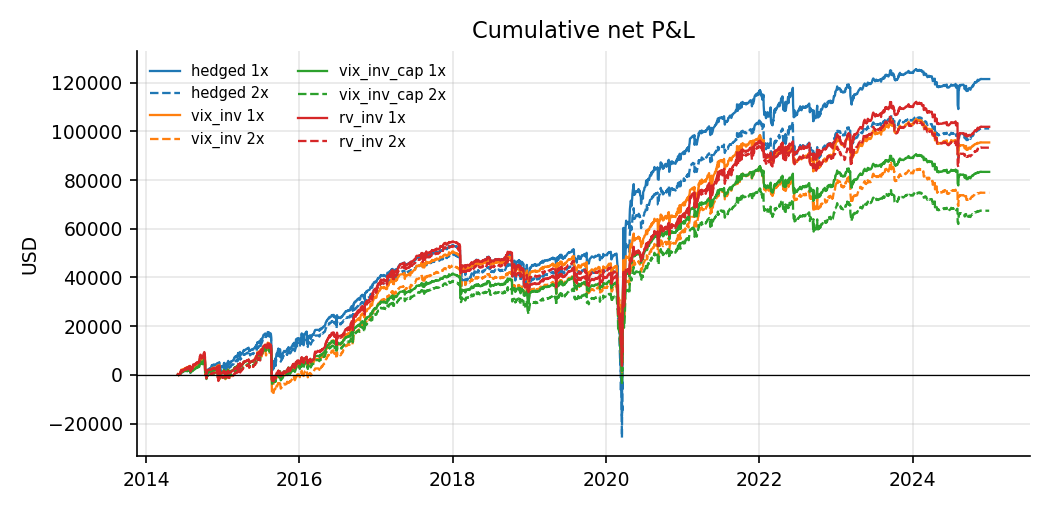
\includegraphics[width=0.92\linewidth]{figures/cum_pnl.png}\caption{Cumulative net P\&L, 1x solid and 2x dashed}\end{figure}

All four books hold the same put on most days: 178 of \texttt{vix\_\allowbreak{}inv}'s 183 entries fall on the same day as an entry of \texttt{hedged}. \texttt{vix\_\allowbreak{}inv} falls behind in August 2015 and in early 2020 and does not catch up. It gains back a little in 2016, 2017 and 2021, when VIX was low and it held more contracts, and in 2018, when it was smaller in the February and December spikes.

\begin{figure}[H]\centering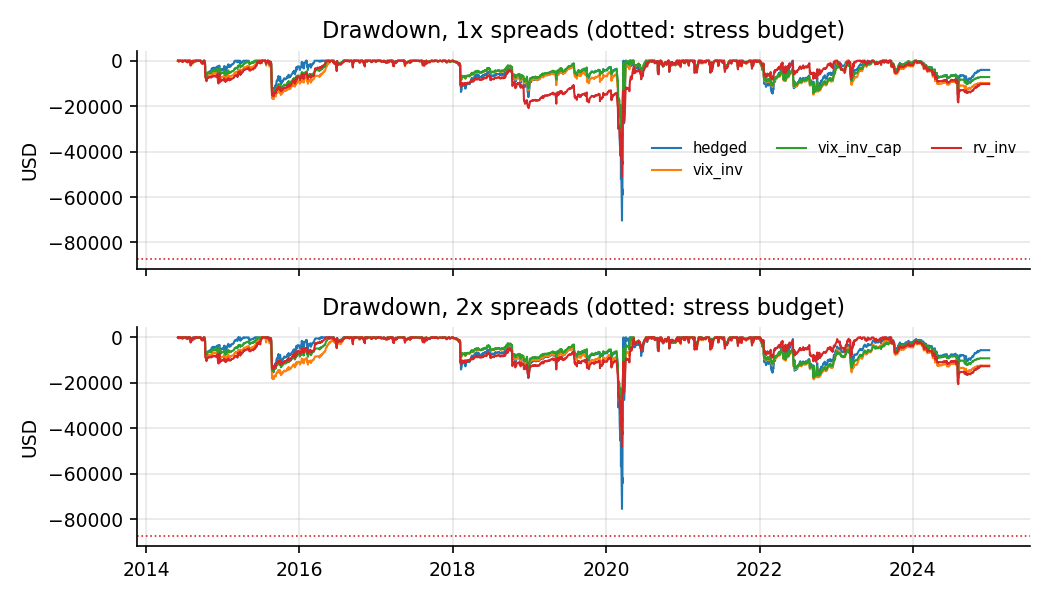
\includegraphics[width=0.92\linewidth]{figures/drawdown.png}\caption{Drawdown at 1x and 2x spreads; dotted line: the \$87,500 stress budget}\end{figure}

Every book's deepest drawdown falls on 17 March 2020. \texttt{vix\_\allowbreak{}inv} loses \$41k there against \texttt{hedged}'s \$70k, because it entered the spike at half size. \texttt{rv\_\allowbreak{}inv} also stays underwater from January 2018, and its drawdown deepens from late 2018 to early 2020. That is path dependence: after a September 2018 profit-take it re-entered on dates the \texttt{hedged} book did not. Its seven round trips entered from mid-September 2018 to early January 2019 on such dates lost about \$15k in total.

\begin{figure}[H]\centering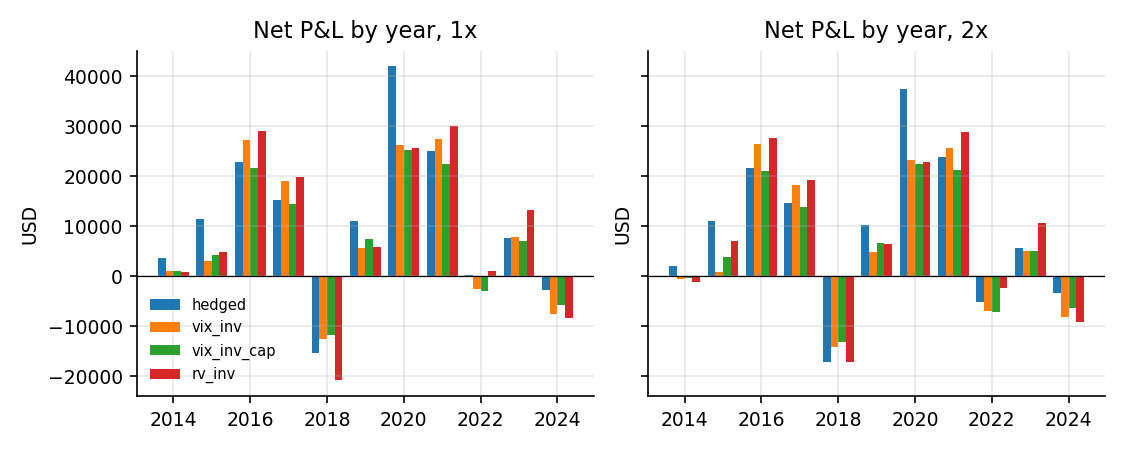
\includegraphics[width=0.92\linewidth]{figures/yearly.png}\caption{Net P\&L by year}\end{figure}

At 1x, \texttt{vix\_\allowbreak{}inv} makes less than \texttt{hedged} in 6 of 11 years. The largest gaps are 2020 (\ensuremath{-}\$15.8k), 2015 (\ensuremath{-}\$8.4k), 2019 (\ensuremath{-}\$5.4k) and 2024 (\ensuremath{-}\$4.8k). It makes more in 2016, 2017, 2018, 2021 and 2023, by \$0.3k to \$4.4k each.

\begin{figure}[H]\centering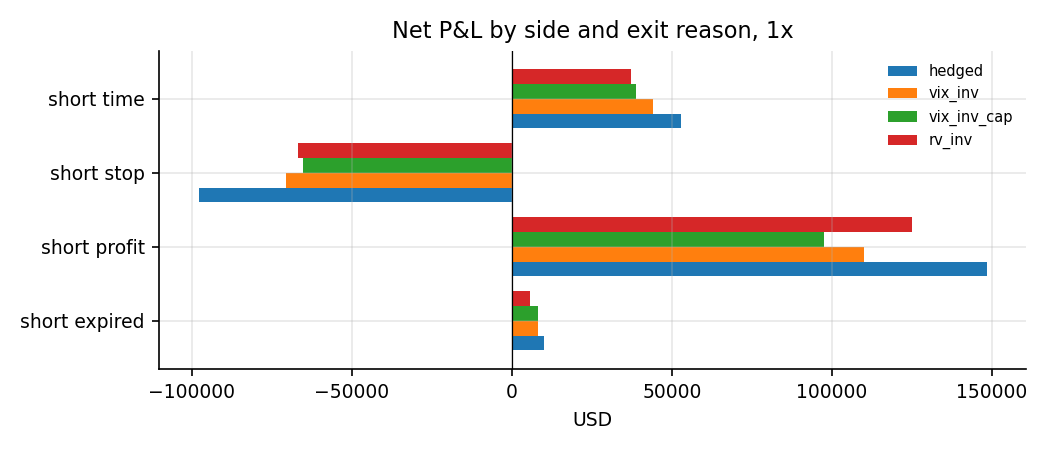
\includegraphics[width=0.92\linewidth]{figures/by_reason.png}\caption{Net P\&L by side and exit reason, 1x}\end{figure}

\texttt{vix\_\allowbreak{}inv} cuts stop losses by \$27.2k, but its profit-takes shrink by \$38.3k and its time exits by \$8.9k. It sold less on stressed days whose puts later paid off.

\begin{figure}[H]\centering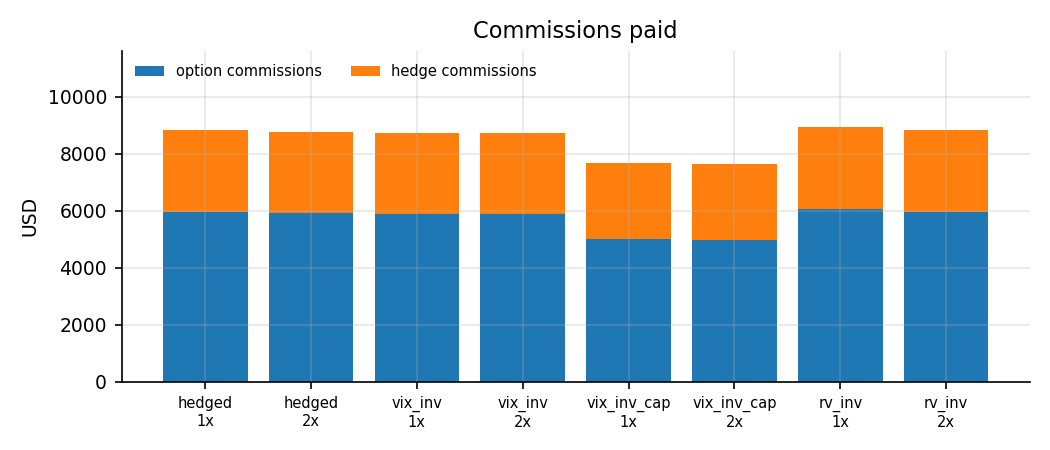
\includegraphics[width=0.92\linewidth]{figures/fees.png}\caption{Commissions paid}\end{figure}

Commissions barely move (about \$8.7k to \$8.9k), except for the capped book, which is smaller on average and pays about \$1.1k less. Costs don't explain the result.

\begin{figure}[H]\centering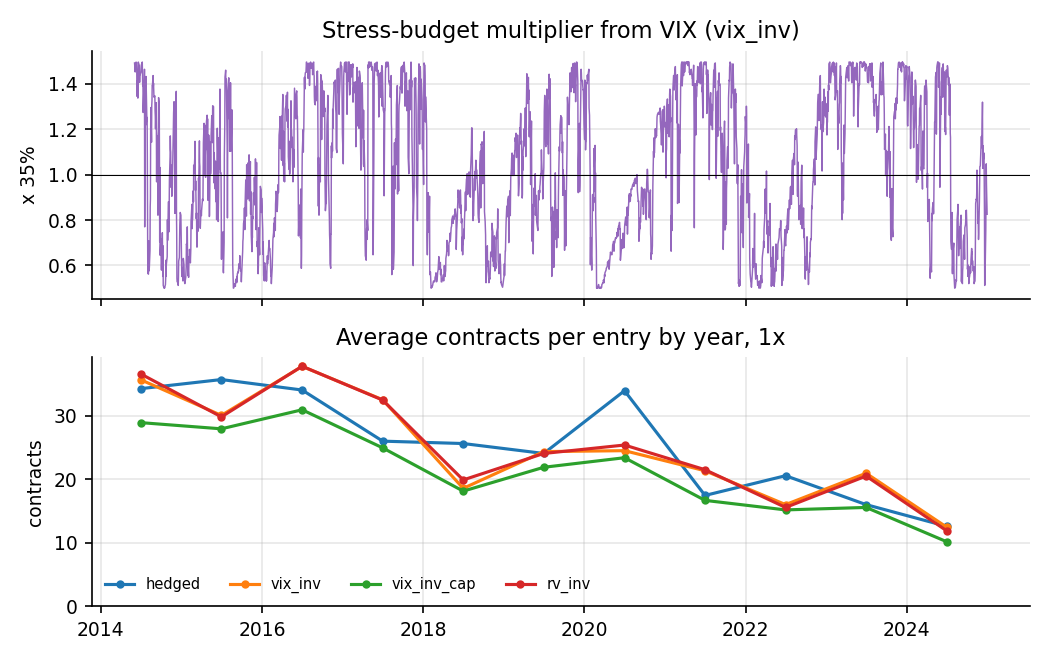
\includegraphics[width=0.92\linewidth]{figures/multiplier.png}\caption{Stress-budget multiplier from VIX's one-year percentile, and average contracts per entry by year}\end{figure}

The multiplier swings between its bounds within weeks, because VIX's percentile moves fast after a spike. Average size at entry is almost unchanged (1.03x mean at entry; 49\% of entries below 1x). The tilt moves size between years: more in 2016-2017, 2021 and 2023; less in 2015, 2018, 2020 and 2022.

\section{Analysis}

\textbf{The Sharpe gain is the March 2020 cut.}

\begin{itemize}

\item All five entries from 26 February to 17 April 2020 came at 0.50x to 0.61x, because VIX was at or near its one-year high at each prior close.

\item The 100- and 71-contract entries of \texttt{hedged} became 49 and 37 contracts.

\item From 19 February to 30 April 2020, \texttt{vix\_\allowbreak{}inv} made \$9.0k against \texttt{hedged}'s \$21.7k at 1x, and its drawdown fell from \$70k to \$41k.

\item Outside that window, \texttt{vix\_\allowbreak{}inv} has a lower Sharpe than \texttt{hedged} (0.75 against 0.81 at 1x) and makes \$86.5k against \$99.8k. The same holds for \texttt{vix\_\allowbreak{}inv\_\allowbreak{}cap} (0.73) and \texttt{rv\_\allowbreak{}inv} (0.78).

\end{itemize}

\textbf{Before 2020 the tilt sized the wrong way around shocks.}

\begin{itemize}

\item A put entered at a calm low VIX is sized up just before a spike. One entered right after a spike is sized down, though those puts are the richest and usually recover.

\item In 2015, the entry in mid-August came at 1.14x and was stopped out. The entry the day after the 24 August spike came at 0.5x and made about half what the \texttt{hedged} entry made.

\item Around the December 2018 selloff the effects cancel: the 14 December entry at 0.65x made less in the year-end rebound (about \ensuremath{-}\$1.6k), while being smaller in the December fall gained \$2.7k. Over December 2018 and January 2019 combined the books are level.

\item In 2014-2019, mean daily P\&L fell 11\% (\$32.3 against \$36.1) and its volatility only 4\%, so the Sharpe fell.

\end{itemize}

\textbf{Per-contract P\&L is highest at low VIX, but the dollars are at high VIX.} In the \texttt{hedged} book, mean net P\&L per contract by multiplier tercile at entry was:

\begin{itemize}

\item \$7.9 in the high-VIX tercile (multiplier about 0.64x);

\item \$1.1 in the middle tercile;

\item \$21.9 in the low-VIX tercile (about 1.40x).

\end{itemize}

So the tilt does put more contracts where the reference earned more per contract. But the high-VIX tercile carried the most dollars (\$71.2k of \$113.2k round-trip net), from a few large crash entries, and the tilt halves those.

The result is mostly mechanical: a smaller book in the crash. The yearly differences outside 2020 are a few thousand dollars and change sign, so the evidence of timing skill either way is weak.

\section{Verdict}

\textbf{Failed}, per the pre-registered bar: Sharpe in 2014-2019 is lower at both 1x and 2x. The tilt behaves like a smaller budget in crashes, as the slope-sizing card found, and it trails the fixed budget outside March 2020. Archive the card and don't run the hold-out. The 15\% and 25\% budgets and the 1.5\ensuremath{\times}IV stress (\texttt{2026-\allowbreak{}11-\allowbreak{}02-\allowbreak{}crash-\allowbreak{}shock}) are the direct test of cutting crash size.

\section{Caveats}

\begin{itemize}

\item \textbf{In-sample:} the book was chosen after its 2014-2024 results, and earlier cards on it (slope sizing, \texttt{vvix\_\allowbreak{}reverse}) had already shown that sizing down in stress raises the full-window Sharpe. Only the hold-out could confirm a result.

\item \textbf{One episode:} the full-window Sharpe and drawdown results rest on five entries in early 2020.

\item \textbf{Rank, not ratio:} the multiple uses VIX's one-year percentile, not 1/\allowbreak{}VIX, so it reverses quickly after a spike. A literal 1/\allowbreak{}VIX ratio might behave differently.

\item \textbf{Spread model:} fitted on about two weeks of calm 2026 live quotes. The 2x run is the stress test, and large March 2020 fills use the same model as small ones.

\item \textbf{Data gaps:} R2 has no month-end weekdays, so about 3.3\% of scheduled times are skipped.

\item \textbf{Margin:} not modelled.

\end{itemize}

\section{Trials}

6 trials for this experiment (3 variants \ensuremath{\times} 1x and 2x, one run of \texttt{experiment.\allowbreak{}py}), plus the baseline's 2. The \texttt{hedged} reference was reused, not rerun. Every row of this run is tagged \texttt{-\allowbreak{}dirty}, and the commit tags differ (3ab834b, af47198, 79b09a1, 3568520). Other cards of the same batch were committing their pre-registrations and writing files in the shared working tree during the run. Each tagged commit contains this card's pre-registration (e31b598) and changes no engine code, \texttt{backtest.\allowbreak{}toml}, or this card's config or files. The pass bar was not changed.

\end{document}
